%% =============================================================
%%  Les intervalles — du demi-ton à l'octave
%%  Guide de référence, composé en LaTeX, gravures LilyPond
%% =============================================================
%%
%%  Les figures (gravures/i-*.cropped.pdf) et le tableau
%%  (gravures/intervalles-table.tex) sont produits par
%%  outils/generer_intervalles.py, à partir du modèle des intervalles
%%  (outils/intervalles.py) — le même que celui des fichiers MusicXML.
%%  Voir le colophon en dernière page.
%%
\documentclass[a4paper,11pt]{article}

\usepackage[top=2.2cm,bottom=2.4cm,left=2.2cm,right=2.2cm]{geometry}
\usepackage[T1]{fontenc}
\usepackage[utf8]{inputenc}
\usepackage[french]{babel}
\usepackage{lmodern}
\usepackage{xcolor}
\usepackage{graphicx}
\usepackage{titlesec}
\usepackage{fancyhdr}
\usepackage{mdframed}
\usepackage{array}
\usepackage{enumitem}
\usepackage{booktabs}
\usepackage{longtable}
\usepackage{hyperref}

\graphicspath{{gravures/}}

% ---- Couleurs, reprises du document des accords de guitare ---------
\definecolor{navy}{RGB}{18,50,105}
\definecolor{lightnavy}{RGB}{235,241,255}
\definecolor{mygray}{RGB}{110,110,110}
\definecolor{accent}{RGB}{150,40,30}

\hypersetup{colorlinks=true, linkcolor=navy, urlcolor=navy,
  pdftitle={Les intervalles — du demi-ton à l'octave},
  pdfauthor={Fabian Bastin}}

% ---- En-tête et pied -----------------------------------------------
\pagestyle{fancy}
\fancyhf{}
\renewcommand{\headrulewidth}{0.4pt}
\renewcommand{\footrulewidth}{0.4pt}
\fancyhead[L]{\small\bfseries\textcolor{navy}{Les intervalles}}
\fancyhead[R]{\small\textcolor{mygray}{\thepage}}
\fancyfoot[C]{\small\textcolor{mygray}{Du demi-ton à l'octave}}

% ---- Titres de section ---------------------------------------------
\newcommand{\navysect}[1]{%
  \colorbox{navy}{%
    \parbox[c][17pt]{\dimexpr\linewidth-2\fboxsep\relax}{%
      \color{white}\hspace{6pt}\bfseries\normalsize #1}}%
}
\titleformat{\section}[block]{\normalfont}{}{0pt}{\navysect}
\titlespacing*{\section}{0pt}{16pt}{10pt}
\titleformat{\subsection}
  {\normalfont\normalsize\bfseries\color{navy}}{\thesubsection}{0.6em}{}
\titlespacing*{\subsection}{0pt}{12pt}{5pt}

% ---- Encadré de remarque -------------------------------------------
\newmdenv[linecolor=navy, linewidth=0.5pt, backgroundcolor=lightnavy,
  innertopmargin=6pt, innerbottommargin=6pt,
  innerleftmargin=8pt, innerrightmargin=8pt,
  skipabove=8pt, skipbelow=8pt]{remarque}

% ---- Figure gravée ---------------------------------------------------
% Les gravures sont rognées au trait par LilyPond ; on les centre sans
% cadre, avec une légende discrète.
% Figure gravée, à la largeur donnée (part de la ligne), avec sa légende.
% Le tout tient dans une minipage : figure et légende ne sont jamais
% séparées par un saut de page.
\newcommand{\gravure}[3]{%
  \par\medskip\noindent
  \begin{minipage}{\linewidth}
    \centering
    \includegraphics[width=#2\linewidth]{#1.cropped.pdf}\\[4pt]
    {\small\itshape\color{mygray} #3}
  \end{minipage}\par\medskip
}

% `max width` vient de adjustbox ; à défaut, on se rabat sur width.
\usepackage[export]{adjustbox}

\setlist{itemsep=2pt, topsep=4pt, parsep=0pt}

\begin{document}

% =====================================================================
\begin{titlepage}
\centering
\vspace*{3cm}
{\Huge\bfseries\color{navy} Les intervalles\par}
\vspace{0.6cm}
{\LARGE\color{navy} Du demi-ton à l'octave\par}
\vspace{1.4cm}
{\large Nommer, mesurer, renverser\par}
\vspace{2.5cm}
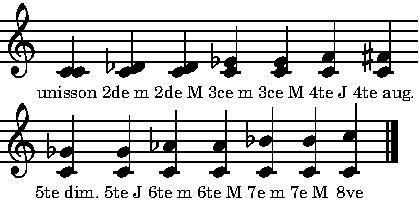
\includegraphics[width=0.7\linewidth]{i-sur-do.cropped.pdf}
\vfill
{\small\color{mygray}
Gravures LilyPond, composition \LaTeX.\\
Fichiers MusicXML joints.\par}
\vspace{1cm}
\end{titlepage}

\tableofcontents
\newpage

% =====================================================================
\section{Avant-propos}

Un \textbf{intervalle} est la distance entre deux notes. Son nom en dit plus
que le simple nombre de demi-tons qui les sépare.

À lire avant
\href{https://www.slashbin.net/musique/theorie/gammes.pdf}{\emph{Les gammes
— construction par tétracordes}}, qui emploie les intervalles sans les
redéfinir : la quarte juste que couvre un tétracorde, la quinte du cycle des
quintes, le triton du tétracorde lydien, la seconde augmentée de la mineure
harmonique. Tout ce qu'il faut pour le lire se trouve ici. Le guide
\href{https://www.slashbin.net/musique/theorie/frequences.pdf}{\emph{Les
fréquences — de l'octave au comma}} dit ensuite ce que mesurent ces
intervalles : des rapports de fréquences, à vérifier à l'oreille au
synthétiseur.

\begin{remarque}
\textbf{Conventions.} Les notes sont nommées en français (do, ré, mi, fa,
sol, la, si). Le \emph{demi-ton} est le plus petit intervalle du système
tempéré ; le \emph{ton} en vaut deux. Un intervalle est \emph{mélodique}
quand ses deux notes se suivent, \emph{harmonique} quand elles sonnent
ensemble ; il porte le même nom dans les deux cas. Sauf mention contraire,
on le mesure de la note grave à la note aiguë.
\end{remarque}

Les fichiers MusicXML qui accompagnent ce document font entendre chaque
intervalle, joué note après note puis les deux notes ensemble ; la
section~\ref{sec:musicxml} les présente.

% =====================================================================
\section{Un nom en deux parties}
\label{sec:nom}

Le nom d'un intervalle a deux parties, qui ne se mesurent pas de la même
façon.

\textbf{Le numéro se compte en lettres.} On compte les noms de notes de la
grave à l'aiguë, les deux comprises : de do à mi, on passe par do, ré, mi —
trois lettres, c'est une \emph{tierce}. Les altérations n'y changent rien :
do--mi, do--mi bémol et do dièse--mi bémol sont toutes des tierces. Le même
nom de note répété est un \emph{unisson} (1), la même lettre huit degrés plus
haut une \emph{octave} (8).

\textbf{La qualité se compte en demi-tons.} Elle distingue les intervalles de
même numéro : do--mi, quatre demi-tons, est une tierce \emph{majeure} ; do--mi
bémol, trois demi-tons, une tierce \emph{mineure}.

\gravure{i-compter}{0.55}{Le numéro se lit sur les lettres, la qualité sur les
demi-tons. Do--mi bémol et do--ré dièse ont la même taille, trois demi-tons,
mais pas le même nom : l'un enjambe trois lettres, l'autre deux.}

\begin{remarque}
\textbf{Le numéro compte les degrés.} On compte les lettres pour la raison qui
oblige à écrire fa dièse et non sol bémol en sol majeur : une gamme emploie
chaque lettre une
fois et une seule. Entre deux degrés voisins d'une gamme, il y a donc toujours
une \emph{seconde} — même quand ils sont à un ton et demi, comme fa et sol dièse
en la mineur harmonique. Le numéro d'un intervalle dit combien de degrés il
enjambe ; la qualité, de combien de demi-tons.
\end{remarque}

On compte les deux extrémités : c'est pourquoi l'octave, qui monte de sept
lettres, porte le numéro huit, et l'unisson, qui ne monte pas, le numéro un.
Cette habitude a une conséquence que l'on retrouve plus loin : les numéros ne
s'additionnent pas simplement (section~\ref{sec:renversement}).

% =====================================================================
\section{Les deux familles}
\label{sec:familles}

Les numéros se partagent en deux familles, qui n'emploient pas les mêmes
qualités.

\textbf{Les intervalles justes} : l'unisson, la quarte, la quinte et l'octave.
Leur forme usuelle est dite \emph{juste} — ni majeure ni mineure. La quarte
juste compte cinq demi-tons, la quinte juste sept.

\textbf{Les intervalles majeurs ou mineurs} : la seconde, la tierce, la sixte
et la septième. Chacun a deux formes usuelles, la mineure plus petite d'un
demi-ton que la majeure.

La gamme majeure montre d'où vient ce partage. Entre ses degrés, toutes les
quintes sont justes sauf une (si--fa), toutes les quartes aussi sauf une
(fa--si) : la quinte et la quarte n'y ont qu'une forme courante. Les tierces,
elles, s'y présentent sous deux formes — majeures sur do, fa et sol,
mineures sur ré, mi, la et si — et les secondes, les sixtes et les
septièmes aussi.

\textbf{Augmenté et diminué.} Un intervalle agrandi d'un demi-ton au-delà de
sa forme juste ou majeure est \emph{augmenté} ; réduit d'un demi-ton en deçà
de sa forme juste ou mineure, il est \emph{diminué}. Ainsi do--fa dièse est
une quarte augmentée, do--sol bémol une quinte diminuée.

\begin{remarque}
\textbf{En résumé.} Juste, majeur et mineur sont les formes usuelles ;
augmenté et diminué, les formes plus larges ou plus étroites d'un demi-ton.
Une quarte ne peut pas être majeure, une tierce ne peut pas être juste.
\end{remarque}

\begin{center}
%% Produit par outils/generer_intervalles.py — ne pas modifier à la main.

\begin{tabular}{@{}l l c l l@{}}
\toprule
\textbf{Intervalle} & \textbf{Abrégé} & \textbf{Demi-tons} & \textbf{Sur do} & \textbf{Renversement} \\
\midrule
unisson & unisson & 0 & do -- do & octave \\
seconde mineure & 2de m & 1 & do -- ré bémol & septième majeure \\
seconde majeure & 2de M & 2 & do -- ré & septième mineure \\
tierce mineure & 3ce m & 3 & do -- mi bémol & sixte majeure \\
tierce majeure & 3ce M & 4 & do -- mi & sixte mineure \\
quarte juste & 4te J & 5 & do -- fa & quinte juste \\
quarte augmentée & 4te aug. & 6 & do -- fa dièse & quinte diminuée \\
quinte diminuée & 5te dim. & 6 & do -- sol bémol & quarte augmentée \\
quinte juste & 5te J & 7 & do -- sol & quarte juste \\
sixte mineure & 6te m & 8 & do -- la bémol & tierce majeure \\
sixte majeure & 6te M & 9 & do -- la & tierce mineure \\
septième mineure & 7e m & 10 & do -- si bémol & seconde majeure \\
septième majeure & 7e M & 11 & do -- si & seconde mineure \\
octave & 8ve & 12 & do -- do & unisson \\
\bottomrule
\end{tabular}


\end{center}

\gravure{i-sur-do}{0.9}{Les quatorze intervalles simples au-dessus de do, de
l'unisson à l'octave. La quarte augmentée et la quinte diminuée ont la même
taille, six demi-tons.}

Le tableau ne donne que les formes les plus courantes. Les autres existent :
do dièse--mi bémol est une tierce diminuée (deux demi-tons), do--ré dièse une
seconde augmentée (trois demi-tons).

% =====================================================================
\section{Même son, autre nom}
\label{sec:enharmonie}

Sur un piano, fa--sol dièse et fa--la bémol se jouent avec les mêmes touches.
Pourtant le premier est une seconde augmentée, le second une tierce mineure :
fa--sol dièse enjambe deux lettres, fa--la bémol trois. Deux intervalles de
même taille mais de noms différents sont dits \textbf{enharmoniques}.

\gravure{i-enharmonie}{0.55}{Même son, deux noms : seconde augmentée et tierce
mineure, quarte augmentée et quinte diminuée. C'est l'écriture qui tranche.}

Le nom n'est pas affaire de goût : il suit l'écriture, et l'écriture suit la
gamme. En la mineur harmonique, le septième degré est sol dièse — la lettre
sol, haussée — et non la bémol, puisque la lettre la est déjà la tonique.
Entre le sixième degré, fa, et ce sol dièse s'ouvre donc une seconde
augmentée, et non une tierce mineure : c'est elle qui donne à cette gamme sa
couleur caractéristique.

Le cas le plus célèbre est celui du \textbf{triton}, l'intervalle de trois
tons. Écrit do--fa dièse, c'est une quarte augmentée ; écrit do--sol bémol,
une quinte diminuée. On le rencontre dans le guide des gammes : les quatre
notes fa--sol--la--si du tétracorde lydien couvrent un triton, fa--si, et non
une quarte juste.

% =====================================================================
\section{Le renversement}
\label{sec:renversement}

\textbf{Renverser} un intervalle, c'est faire passer sa note grave à l'octave
supérieure : do--mi devient mi--do. Les deux notes restent les mêmes, mais
l'intervalle change de nom, selon trois règles.

\begin{remarque}
\textbf{Les numéros se complètent à neuf}, \textbf{les qualités s'échangent}
(majeure et mineure, augmentée et diminuée ; la juste reste juste), et
\textbf{les tailles se complètent à douze demi-tons}.
\end{remarque}

Ainsi la tierce majeure do--mi devient la sixte mineure mi--do : 3~+~6~=~9,
et 4~+~8~=~12 demi-tons. La quinte juste do--sol devient la quarte juste
sol--do.

\gravure{i-renversements}{0.9}{Chaque intervalle suivi de son renversement, la note
grave passée à l'octave.}

Pourquoi neuf et non huit ? Parce que la note commune, mi, est comptée deux
fois : de do à mi, trois lettres ; de mi à do, six ; mais mi appartient aux
deux décomptes.

Le renversement éclaire deux faits du guide des gammes.

\begin{itemize}
  \item La \textbf{sous-dominante} est une quinte \emph{au-dessous} de la
    tonique : fa, quinte juste sous do, est aussi une quarte juste au-dessus.
    Les deux descriptions désignent la même note, à l'octave près.
  \item \textbf{Monter d'une quinte revient à descendre d'une quarte.} C'est
    pourquoi le cycle des quintes, parcouru à l'envers, est un cycle des
    quartes : les bémols s'ajoutent en montant de quarte en quarte.
\end{itemize}

Enfin, le triton est le seul intervalle qui reste le même en se renversant :
six demi-tons, et six pour le compléter à l'octave. Quarte augmentée et
quinte diminuée sont l'une le renversement de l'autre. Il partage l'octave en
deux moitiés égales.

% =====================================================================
\section{Les intervalles de la gamme majeure}
\label{sec:majeure}

Mesurés depuis la tonique, tous les intervalles de la gamme majeure sont
\emph{majeurs} ou \emph{justes} : seconde, tierce, sixte et septième majeures,
quarte et quinte justes, octave.

\gravure{i-gamme-majeure}{0.7}{De la tonique de do majeur à chacun de ses degrés :
tous les intervalles sont majeurs ou justes.}

« Majeur » et « juste » désignent donc exactement les intervalles de la gamme
majeure lus depuis sa tonique — un repère commode, dont on tire une méthode
pour qualifier n'importe quel intervalle.

\begin{remarque}
\textbf{Pour qualifier un intervalle}, imaginer la gamme majeure de sa note
grave. Si la note aiguë en fait partie, l'intervalle est majeur ou juste. Si
elle est un demi-ton plus bas, il est mineur (ou diminué, pour un juste) ; un
demi-ton plus haut, augmenté.
\end{remarque}

Par exemple, mi--do : la gamme de mi majeur a do dièse pour sixième degré ;
do est un demi-ton plus bas, mi--do est donc une sixte mineure — comme l'a
montré le renversement de do--mi.

Les intervalles entre degrés voisins retrouvent le vocabulaire du guide des
gammes : le ton est une seconde majeure, le demi-ton une seconde mineure. Un
tétracorde couvre une quarte juste, et les deux tétracordes d'une gamme
majeure commencent à une quinte juste l'un de l'autre, sur la tonique et sur
la dominante.

% =====================================================================
\section{Consonance et dissonance}
\label{sec:consonance}

Joués ensemble, certains intervalles sonnent reposés, d'autres tendus. La
tradition les classe ainsi :

\begin{itemize}
  \item \textbf{consonances parfaites} : l'unisson, l'octave, la quinte juste,
    et la quarte juste — que l'harmonie classique traite toutefois comme une
    dissonance lorsqu'elle se forme au-dessus de la basse ;
  \item \textbf{consonances imparfaites} : les tierces et les sixtes,
    majeures ou mineures ;
  \item \textbf{dissonances} : les secondes, les septièmes, et les
    intervalles augmentés ou diminués, triton compris.
\end{itemize}

Les consonances parfaites sont celles dont les fréquences sont dans les
rapports les plus simples : 2 pour 1 à l'octave, 3 pour 2 à la quinte, 4 pour
3 à la quarte. Le tempérament égal, qui partage l'octave en douze demi-tons
égaux, les approche plus ou moins bien : il respecte exactement l'octave,
manque la quinte et la quarte de deux centièmes de demi-ton à peine, mais les
tierces et les sixtes de quatorze à seize centièmes. Le guide
\href{https://www.slashbin.net/musique/theorie/frequences.pdf}{\emph{Les
fréquences}} détaille ces rapports, d'où viennent le ton, le demi-ton et le
comma, et comment le tempérament égal s'en accommode.

% =====================================================================
\section{Au-delà de l'octave}
\label{sec:composes}

Un intervalle plus grand qu'une octave est dit \textbf{composé}. Il se nomme
comme l'intervalle simple qu'il contient, augmenté d'une octave : la neuvième
est une octave plus une seconde, la dixième une octave plus une tierce, et
ainsi de suite. Il garde la qualité de l'intervalle simple : do--ré de
l'octave suivante est une neuvième majeure, comme do--ré est une seconde
majeure.

La règle des numéros est celle du renversement : la note commune compte deux
fois, et l'on retire un. Une octave plus une seconde fait 8~+~2~--~1~=~9.
Les intervalles composés sont courants dans l'écriture des accords, où l'on
parle de neuvième, de onzième ou de treizième.

% =====================================================================
\section{Les fichiers MusicXML}
\label{sec:musicxml}

Les fichiers joints se lisent avec MuseScore, Finale, Sibelius, Dorico ou tout
éditeur de partitions ; sur slashbin.net, ils s'écoutent aussi dans Sodor
Piano. Chaque intervalle y est joué note après note, puis les deux notes
ensemble, et porte son nom au-dessus de la portée.

\begin{itemize}
  \item \texttt{intervalles.musicxml} — les quatorze intervalles simples
    au-dessus de do, de l'unisson à l'octave ;
  \item \texttt{intervalles-gamme-majeure.musicxml} — de la tonique de do
    majeur à chacun de ses degrés ;
  \item \texttt{intervalles-renversements.musicxml} — cinq intervalles, chacun
    suivi de son renversement.
\end{itemize}

% =====================================================================
\section*{Colophon}
\addcontentsline{toc}{section}{Colophon}

Les gravures musicales sont produites par \textbf{LilyPond}, la composition
par \textbf{\LaTeX}. Les figures, le tableau et les fichiers MusicXML sont
dérivés d'un unique modèle, le module \texttt{intervalles.py} du dossier \texttt{outils}, bâti
sur le modèle de hauteurs du guide des gammes : un intervalle y est un couple
(numéro, qualité), comme une hauteur y est un couple (lettre, altération). Le
générateur vérifie que construire un intervalle puis le mesurer redonne le
même nom, et que chaque renversement complète bien l'octave, sur toutes les
toniques des gammes. Pour régénérer l'ensemble :

\begin{center}
\texttt{python3 outils/generer\_intervalles.py}\\
\texttt{lilypond -dcrop --formats=pdf gravures/i-*.ly}\\
\texttt{pdflatex intervalles.tex}
\end{center}

\end{document}
